\documentclass[onecolumn, letterpaper, 12pt]{report}

% insert any packages, environments, counters, etc here
\usepackage{graphicx}
\usepackage{hyperref}

\begin{document}
%insert document contents here

\chapter{Sequence Modeling: Recurrent and Recursive Nets}

\textbf{Recurrent Neural Networks} or RNNs are a family of neural networks for processing sequential data. 

\href{https://www.iro.umontreal.ca/~vincentp/ift3395/lectures/backprop_old.pdf}{Rumelhart et al, 1986a | Learning Representations by Back Propagating Errors}

\begin{quote}
  We describe a new learning procedure, back-propagation, for networks
  of neurone-like units. The procedure repeatedly adjusts the weights
  of the connections in the network so as to minimize a measure of the
  difference between the actual output vector of the net and the
  desired output vector. As a result of the weight adjustments,
  internal 'hidden' units which are not part of the input or output
  come to represent important features of the task domain, and the
  regularities in the task are captured by the interactions of these
  units. The ability to create useful new features distinguishes
  back-propagation from earlier, simpler methods such as the
  perceptron-convergence procedure.
\end{quote}

A RNN is a network that is specialized for processing a sequence of values $x^{(1)}, ..., x^{(\tau)}$. RNNs can scale to much longer sequences than would be practical for networks without sequence based specialization, and they can also process sequences of variable length. 

To go from multilayer networks to recurrent networks, we need to take advantage of parameter sharing. This makes it possible to extend and apply the model to examples of different forms and generalize across them. Such sharing is important when a specific piece of information can occur at multiple positions within the sequence.

A related idea is the use of convolution across a 1D temporal space. This approach is the basis for time delay neural networks. The convolution operation allows a network to share parameters across time, but it is shallow. The output of convolution is a sequence where each member of the output is a function of a small number of neighboring members of the input. The idea of parameter sharing in this case manifests in the application of the same convolution kernel at each time step.

Recurrent networks share parameters in a different way. Each member of the output is a function of the previous members of the output. Each output member is produced using the same update rule applied to the previous outputs. This formulation results in the sharing of parameters through a very deep computational graph. 

This chapter extends the idea of a computational graph to include cycles which represent the influence of the present value of a variable on its own value at a future time step. 

For more information on recurrent neural networks than is available in this chapter, look into \href{https://www.cs.toronto.edu/~graves/preprint.pdf}{Alex Graves | Supervised Sequence Labelling with Recurrent Neural Networks}

\section{Unfolding Computational Graphs}

In this section we explain the idea of \textbf{unfolding} a recursive or recurrent computation into a computational graph that has a repetitive structure, typically corresponding to a chain of events. Unfolding this graph results in the sharing of parameters across a deep network structure. 

Consider the classical form of a dynamical system: 

\begin{center}
  $s^{(t)} = f(s^{(t-1)}; \theta)$
\end{center}

where $s^{(t)}$ is the state of the system. This is recurrent because the definition of $s$ at time $t$ refers back to the same definition at time $t-1$. 

For a finite number of steps, we can unfold the graph by applying the definition $\tau - 1$ times. For example, if we unfold above 3 times:

\begin{center}
  $s^{(3)} = f(s^{(2)}; \theta) = f(f(s^{(1)}; \theta) \theta)$
\end{center}

By unfolding this repeatedly, we yield an expression that does not involve recurrence. Such an expression can now be represented by a traditional directed acyclic computational graph. 

\begin{figure}[h]
  \centering
  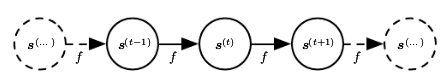
\includegraphics[width=0.7\textwidth]{trad_dag.png}
\end{figure}

Many recurrent networks also define their hidden units using recursive functions, such as 

\begin{center}
  $h^{(t)} = f(h^{(t-1)}, x^{(t)}; \theta)$
\end{center}

Typical RNNs will add extra architectural features such as output layers that read information out of the state $h$ to make predictions. When the network is trained to perform a task that requires predicting the future from the past, the network typically learns to use $h^{(t)}$ as a kind of lossy summary of the task relevant aspects of the past sequence of inputs up to $t$. This summary is in general necessarily lossy since it maps an arbitrary length sequence $(x^{(t)}, x^{(t-1)}, ..., x^{(2)}, x^{(1)})$ to a fixed length vector $h^{(t)}$. 

For example, if we were to use an RNN to predict the next word given the previous words, it may not be necessary to store all of the information in the input sequence up to time t, but instead only enough information to predict the rest of the sentence. The most demanding situation is when we ask $h^{(t)}$ to be rich enough to allow one to approximately recover the input sequence, as in autoencoder frameworks. 

\begin{figure}[h]
  \centering
  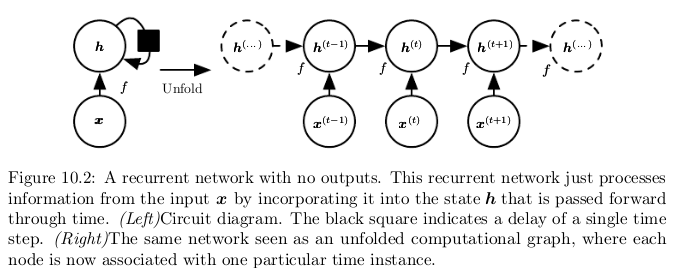
\includegraphics[width=0.7\textwidth]{rnn_dag.png}
\end{figure}

What we call unfolding is the operation that maps a circuit (as in the left side of above) to a computational graph with repeated pieces (as in the right side). The unfolded graph now has a size that depends on the sequence length. 

The unfolding process has two major advantages:

1. Regardless of the sequence length, the learned model always has the same input size, because it is specified in terms of transition from one state to another state, rather than specified in terms of a variable length history of states.

2. It is possible to use the same transition function $f$ with the same parameters at each step

2 follows because we can represent the unfolded recurrence after $t$ steps with a function $g$: 

\begin{center}
  $h^{(t)} = g^{(t)}(x^{(t)}, x^{(t-1)}, ..., x^{(2)}, x^{(1)}) = f(h^{(t-1)}x^{(t)}; \theta)$
\end{center}

The function $g^{(t)}$ takes the whole past sequence as input and produces the current state, but the unfolded recurrent structure allows us to factorize $g^{(t)}$ into repeated applications of a function $f$. 

The two advantages above allow us to learn a single model $f$ that operates on all time steps and all sequence lengths, rather than needing to learn a separate model $g^{(t)}$ for all possible time steps. Learning a single, shared model allows generalization to sequence lengths that did not appear in the training set and allows the model tobe estimated with far fewer training examples than would be required without parameter sharing. 

\section{Recurrent Networks}

Now that we know of graph unrolling and parameter sharing, we can design a wide variety of networks. Some examples of design patterns for RNNs include the following:

- RNNs that produce an output at each time step and have recurrent connections between hidden units

\begin{figure}[h]
  \centering
  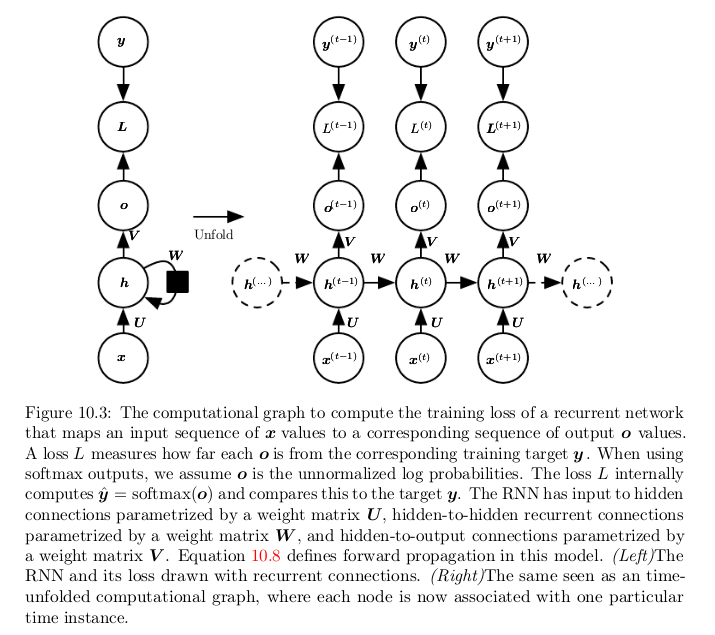
\includegraphics[width=0.7\textwidth]{rnn_dp_1.png}
\end{figure}


- RNNs that produce an output at each time step and have recurrent connections only from the output at one time step to the hidden units at the next time step 

\begin{figure}[h]
  \centering
  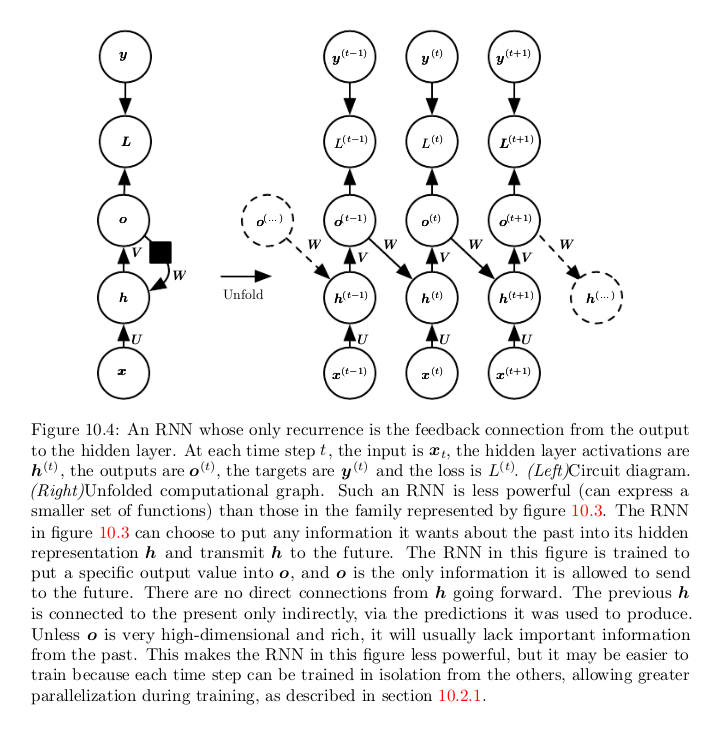
\includegraphics[width=0.7\textwidth]{rnn_dp_2.png}
\end{figure}

- RNNs with recurrent connections between hidden units that read an entire sequence and then produce a single output 

\begin{figure}[h]
  \centering
  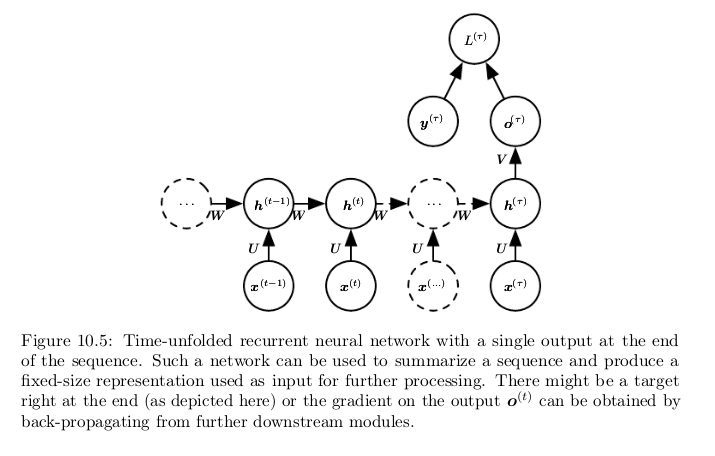
\includegraphics[width=0.7\textwidth]{rnn_dp_3.png}
\end{figure}


\end{document}



